
Some objects don't have a specific length. To know their length, you need to iterate through all their elements. For example, elsewhere in this chapter we've seen a generator that doesn't have a specific length. A more common example would be a C-string.

A C-string is a primitive C-array of characters, terminated with a null '\verb|\|0' value.


\hspace*{\fill} \\ %插入空行
\begin{center}
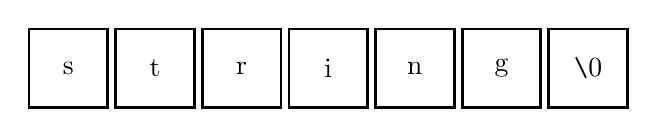
\begin{tikzpicture}
\draw[line width=1pt] (1.1*0,1) rectangle (1.1*0+1,0) node[pos=.5] {s};
\draw[line width=1pt] (1.1*1,1) rectangle (1.1*1+1,0) node[pos=.5] {t};
\draw[line width=1pt] (1.1*2,1) rectangle (1.1*2+1,0) node[pos=.5] {r};
\draw[line width=1pt] (1.1*3,1) rectangle (1.1*3+1,0) node[pos=.5] {i};
\draw[line width=1pt] (1.1*4,1) rectangle (1.1*4+1,0) node[pos=.5] {n};
\draw[line width=1pt] (1.1*5,1) rectangle (1.1*5+1,0) node[pos=.5] {g};
\draw[line width=1pt] (1.1*6,1) rectangle (1.1*6+1,0) node[pos=.5] {\verb|\|0};
\end{tikzpicture}

Figure 4.5 – A C-string with its null terminator
\end{center}

We use C-strings all the time, even if we don't realize it. Any literal string in C/C++ is a C-string:

\begin{lstlisting}[style=styleCXX]
std::string s = "string";
\end{lstlisting}

Here, the STL string s is initialized with a literal string. The literal string is a C-string. If we look at the individual characters in hexadecimal, we'll see the null terminator:

\begin{lstlisting}[style=styleCXX]
for (char c : "string") {
	std::cout << format("{:02x} ", c);
}
\end{lstlisting}

The word "string" has six letters. The output from our loop shows seven elements in the array:

\begin{tcblisting}{commandshell={}}
73 74 72 69 6e 67 00
\end{tcblisting}

The seventh element is the null terminator.

The loop sees the primitive C-array of characters, with seven values. The fact that it's a string is an abstraction invisible to the loop. If we want the loop to treat it like a string, we'll need an iterator and a sentinel.

A sentinel is an object that signals the end of an iterator of indeterminate length. When the iterator hits the end of the data, the sentinel will compare equal with the iterator.

To see how this works, let's build an iterator for C-strings!

\subsubsection{How to do it…}

To use a sentinel with a C-string, we need to build a custom iterator. It doesn't need to be complicated, just the essentials for use with a range-based for loop.

\begin{itemize}
\item 
We'll start with a couple of convenience definitions:

\begin{lstlisting}[style=styleCXX]
using sentinel_t = const char;
constexpr sentinel_t nullchar = '\0';
\end{lstlisting}

The using alias for sentinel\_t is const char. We'll use this for the sentinel in our class.

We also define the constant nullchar for the null character terminator.

\item 
Now we can define our iterator type:

\begin{lstlisting}[style=styleCXX]
class cstr_it {
	const char *s{};
public:
	explicit cstr_it(const char *str) : s{str} {}
	char operator*() const { return *s; }
	cstr_it& operator++() {
		++s;
		return *this;
	}
	bool operator!=(sentinel_t) const {
		return s != nullptr && *s != nullchar;
	}
	cstr_it begin() const { return *this; }
	sentinel_t end() const { return nullchar; }
};
\end{lstlisting}

This is short and simple. It's the minimum necessary for a range-based for loop. Notice the end() function returns a nullchar and the operator!=() overload compares against the nullchar. That's all we need for the sentinel.

\item 
Now we can define a function for printing our C-string using the sentinel:

\begin{lstlisting}[style=styleCXX]
void print_cstr(const char * s) {
	cout << format("{}: ", s);
	for (char c : cstr_it(s)) {
		std::cout << format("{:02x} ", c);
	}
	std::cout << '\n';
}
\end{lstlisting}

In this function we first print the string. Then we use the format() function to print each individual character as a hexadecimal value.

\item 
Now we can call print\_cstr() from our main() function:

\begin{lstlisting}[style=styleCXX]
int main() {
	const char carray[]{"array"};
	print_cstr(carray);
	const char * cstr{"c-string"};
	print_cstr(cstr);
}
\end{lstlisting}

The output looks like this:

\begin{tcblisting}{commandshell={}}
array: 61 72 72 61 79
c-string: 63 2d 73 74 72 69 6e 67
\end{tcblisting}

Notice that there are no extraneous characters and no null terminators. This is because our sentinel tells the for loop to stop when it sees the nullchar.

\end{itemize}

\subsubsection{How it works…}

The sentinel part of the iterator class is very simple. We can easily use the null terminator as the sentinel value by returning it in the end() function:

\begin{lstlisting}[style=styleCXX]
sentinel_t end() const { return nullchar; }
\end{lstlisting}

Then the not-equal comparison operator can test for it:

\begin{lstlisting}[style=styleCXX]
bool operator!=(sentinel_t) const {
	return s != nullptr && *s != nullchar;
}
\end{lstlisting}


Notice that the parameter is just a type (sentinel\_t). A parameter type is necessary for the function signature, but we don't need the value. All that's necessary is to compare the current iterator with the sentinel.

This technique should be useful whenever you have a type or class that doesn't have a predetermined end point for comparison.



















